\documentclass[12pt]{amsart}

\usepackage{latexsym}
\usepackage{amsmath}
\usepackage{amsfonts}
\usepackage{amssymb}
\usepackage{graphicx}

\graphicspath{{images/}}

\newtheorem{theorem}{Theorem}[section]
\newtheorem{lemma}[theorem]{Lemma}
\newtheorem{corollary}[theorem]{Corollary}
\newtheorem{proposition}[theorem]{Proposition}
\newtheorem{noname}[theorem]{}
\newtheorem{sublemma}{}[theorem]
\newtheorem{conjecture}[theorem]{Conjecture}

\theoremstyle{definition}
\newtheorem{definition}[theorem]{Definition}
\newtheorem{example}[theorem]{Example}

\theoremstyle{remark}
\newtheorem{remark}[theorem]{Remark}

\numberwithin{equation}{section}

\newcommand{\bb}[1]{\mathbb{#1}}
\newcommand{\ds}{.3}

\begin{document}

\title{TriColorings of Knots}


\author{Lucas Meyers}
\address{Mathematics Department\\
Louisiana State University\\
Baton Rouge, Louisiana}
\email{lmeye22@lsu.edu}

\subjclass[2010]{57M25}
\date{\today}

\begin{abstract}
  Tricoloring is a knot invariant that differentiates knots
  based on whether or knot their diagram can be colored in a
  certain way with three colors. In this paper, we introduce knots
  and define tricolorability in terms of both knot diagrams
  and the knot group. We then mention extensions of the notions
  of tricolorability to arbitrary $n$-coloring.
\end{abstract}

\maketitle

\section{Introduction}
\label{introduction}

One common pattern we see in mathematics is a concern with how
certain objects fit inside other objects. Knot theory studies this
sort of problem. Given a circle $S^1$ what different ways can we embed
it into $\bb{R}^3$ or $S^3$ ($\bb{R}^3$ with a point at $\infty$)?
A typical drawing of a knot can be seen in Figure~\ref{fig:figure-eight}.



Naturally, once we begin to consider knots, we are also led to consider
how we might tell them apart or rather when they should be the same
at all. Intuitively, the knot in Figure~\ref{fig:figure-eight} should
be considered the same as that in Figure~\ref{fig:figure-eight-t} but should be
different from that of trefoil seen in Figure~\ref{fig:trefoil}. In
the next section, we will see the definition of a knot, how to define their
equivalence in a sensible way, followed by a method to differentiate them
called tricolorability. Afterwards, we will look at an alternative definition
of tricolorability that utilizes the fundamental group.
Then we will introduce notions of how one may consider
coloring knots with more than three colors.

\begin{figure}
  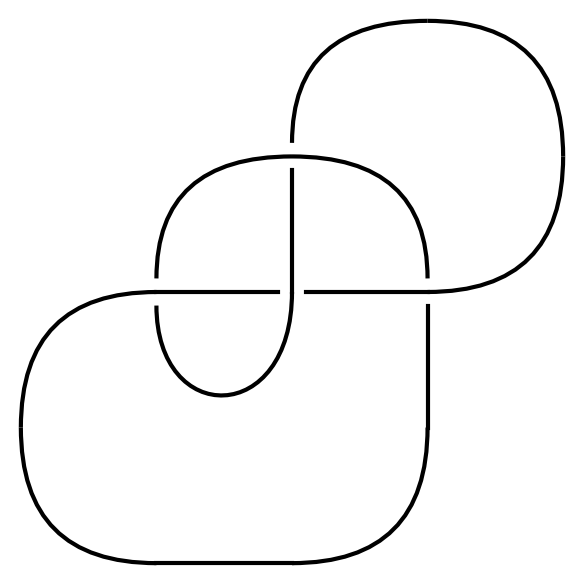
\includegraphics[scale=\ds]{figure-eight}
  \caption{Figure-eight knot}
  \label{fig:figure-eight}
\end{figure}

\begin{figure}
  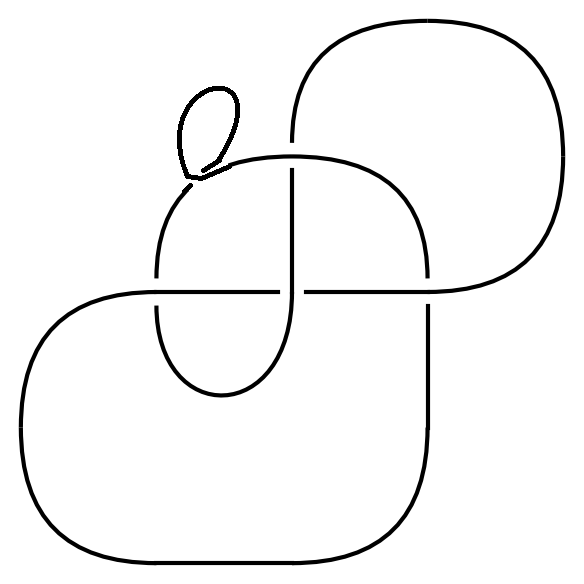
\includegraphics[scale=\ds]{figure-eight-t}
  \caption{Figure-eight with a twist}
  \label{fig:figure-eight-t}
\end{figure}

\section{Diagrams and Coloring}
\label{sec:diagrams-coloring}

In this paper we will follow the conventions of Charles
Livingston~\cite{Livingston}. To begin, we give the definition of a knot.

\begin{definition}
  A \textit{knot} is a simple closed curve in $\bb{R}^3$(or $S^3$).
\end{definition}

Now there are two issues that we need to consider before moving forward.
The first is our notion of equivalence. Unfortunately, a homeomorphism from
one knot to another is too weak a notion of equivalence as all simple closed curves
are homeomorphic to $S^1$. Instead we will use the following: 

\begin{definition}
  Two knots $K$ and $J$ are \textit{ambient isotopic} if there is a homotopy on the ambient
  space $H:S^3\times [0,1]\rightarrow S^3$ if $H(x,0)$ is the identity and the
  image $H(K,1)=J$.
\end{definition}

The second issue of initial concern is that we will be considering a subset of knots called tame. A knot
is \textit{tame} if it is ambient isotopic to a piecewise linear knot. A
knot that is not tame is called \textit{wild} and a drawing of an example of such a knot
seen in Figure~\ref{fig:wild}. The knot in question has a decreasing sequence of
components that cannot be made linear. Wild knots have some more pathological
properties and to keep things simple and consistent we will restrict ourselves to
tame knots.

\begin{figure}
  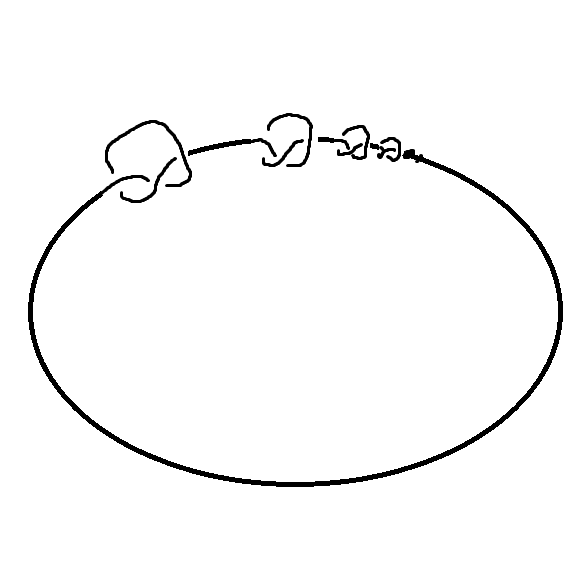
\includegraphics[scale=\ds]{wild}
  \caption{Wild knot}
  \label{fig:wild}
\end{figure}

When we give the initial definition of  tricolorability we will not work
directly with the curves themselves. Instead we will deal with diagrams
of the knots. All drawings of knots in this paper are examples of diagrams.

\begin{definition}
  A \textit{diagram} $D$ for a knot $K$ is a projection of $K$ to a plane
  such that:
  \begin{itemize}
  \item At most two points are sent to the same location on the plane.
    These are called \textit{crossings}.
  \item Given any two crossings they each have an open neighborhood
    that is disjoint from the other's neighborhood.
  \item All crossings must be either overcrossings or undercrossings.
  \end{itemize}
  Note that all figures in this paper are diagrams of knots.
\end{definition}

When we project to a plane there is a loss of information that occurs. This
is why we must denote all crossings as either overcrossings or undercrossings.
This allows one to recover the knot in its entirety from the diagram. Otherwise
it would be ambiguous what knot is recovered since we would have to make a choice
of over or under for each crossing. The segments that make up the diagram
are called \textit{arcs}.

There is one other unfortunate occurrence
from moving to diagrams. It is that there are infinitely many diagrams
for a given knot. Moreover actually telling whether two diagrams denote
the same knot is extremely difficult, though decidable, and moreover
belongs to NP~\cite{Poonen}.

It turns out that there are three ``moves'' along with planar isotopy
that we can apply to diagrams that will allow us to completely characterize
when two diagrams correspond to the same knot.

\begin{definition}
  The \textit{Reidmeister moves} are the moves labeled in Figure~\ref{fig:reidmeister}.
  They are referred to as type-I, type-II, or type-III moves respectively.

  \begin{figure}
    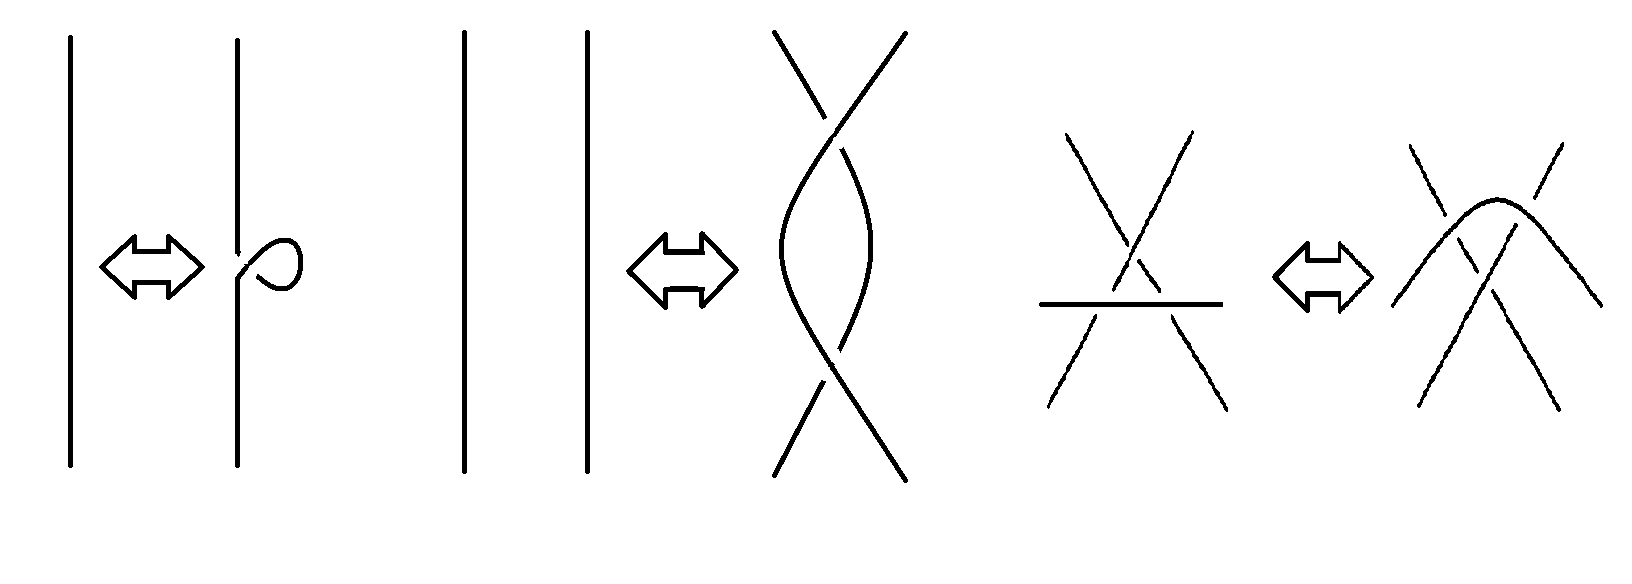
\includegraphics[scale=\ds]{reidmeister}
    \caption{Reidmeister moves of type I, II, and III}
    \label{fig:reidmeister}
  \end{figure}
\end{definition}

We will use, without proof, the following theorem about Reidmeister moves.

\begin{theorem}
  Two knots $K$ and $J$ are ambient isotopic if and only if their diagrams
  are related by a finite sequence of Reidmeister moves and planar isotopy.
\end{theorem}

The importance of Reidmeister moves and diagrams becomes apparent
in defining invariants of knots. If we define an invariant on diagrams and show
that it does not change under planar isotopy or the Reidmeister moves, then
it will also act as an invariant on knots. This is precisely the method we
will use with our initial definition of tricolorability.

There are two knots that we will return to repeatedly
as they are the simplest examples of knots for which tricolorability
differentiates them. The simplest knot is the \textit{unknot} (see Figure~\ref{fig:unknot}), which
is unique in that it has a diagram with no crossings whatsoever. The
other is the \textit{trefoil} shown in Figure~\ref{fig:trefoil}.

\begin{figure}
  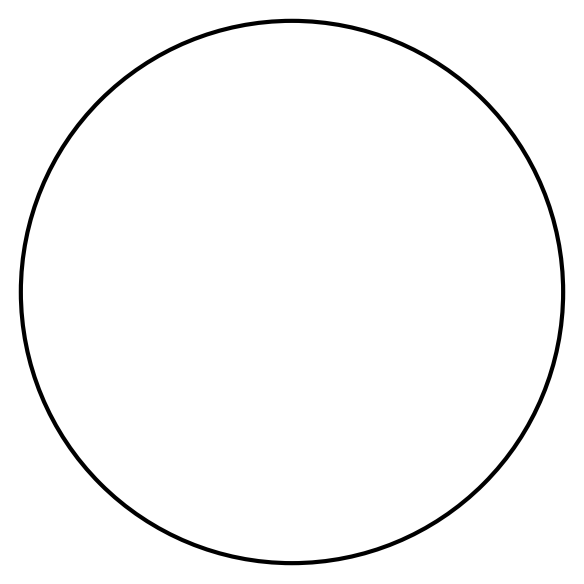
\includegraphics[scale=\ds]{unknot}
  \caption{Unknot}
  \label{fig:unknot}
\end{figure}

\begin{figure}
  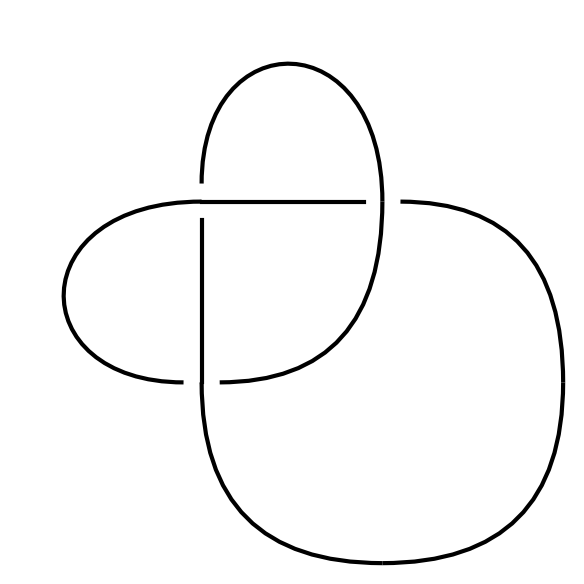
\includegraphics[scale=\ds]{trefoil}
  \caption{Trefoil knot}
  \label{fig:trefoil}
\end{figure}

With that in mind let us introduce tricolorability.

\begin{definition}
  Let $K$ be a knot with diagram $D$. Then a \textit{tricoloring ($3$-coloring)}
  of $K$ is an assignment to each arc one of three colors
  such that at each crossing either all colors appear or
  only single color appears. A tricoloring is called \textit{non-trivial}
  if at least two colors are used.
\end{definition}

We will use the colors red, green, and blue as our colors.
Now we must show that tricoloring is in fact an invariant.

\begin{theorem}
  The existence of a non-trivial $3$-coloring for some diagram is a
  knot invariant.
\end{theorem}

\begin{proof}
  Let $K$ be a knot with diagram $D$. We must show that, given a coloring
  for $D$, we can color any diagram of $K$. First note that planar isotopy
  does not affect the crossings for $D$ and, as such, does not change the
  $3$-colorability.

  Next we will have a series of pictures that demonstrate the possibilities
  for type-I, type-II, and type-III moves respectively.

  For type-I we have there only a single case as a type-I move acts only on
  a single arc as seen in Figure~\ref{fig:t1-c}.
  \begin{figure}
    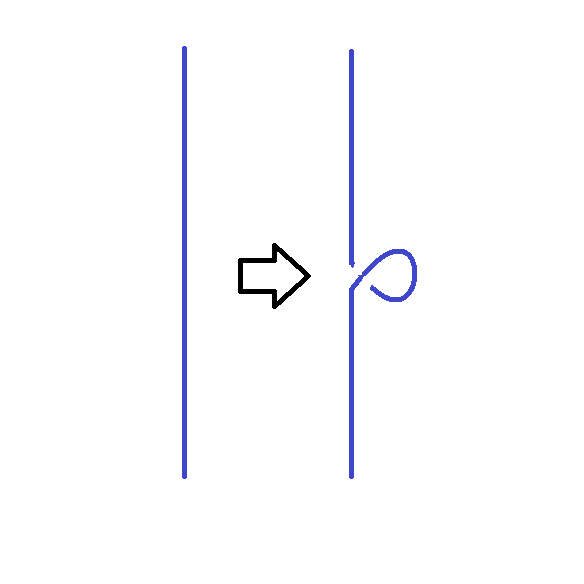
\includegraphics[scale=\ds]{t1-c}
    \caption{type-I}
    \label{fig:t1-c}
  \end{figure}
  
  For type-II, there are two cases either both strands have the same color
  or they are different as seen in Figure~\ref{fig:t2-c}.
  \begin{figure}
    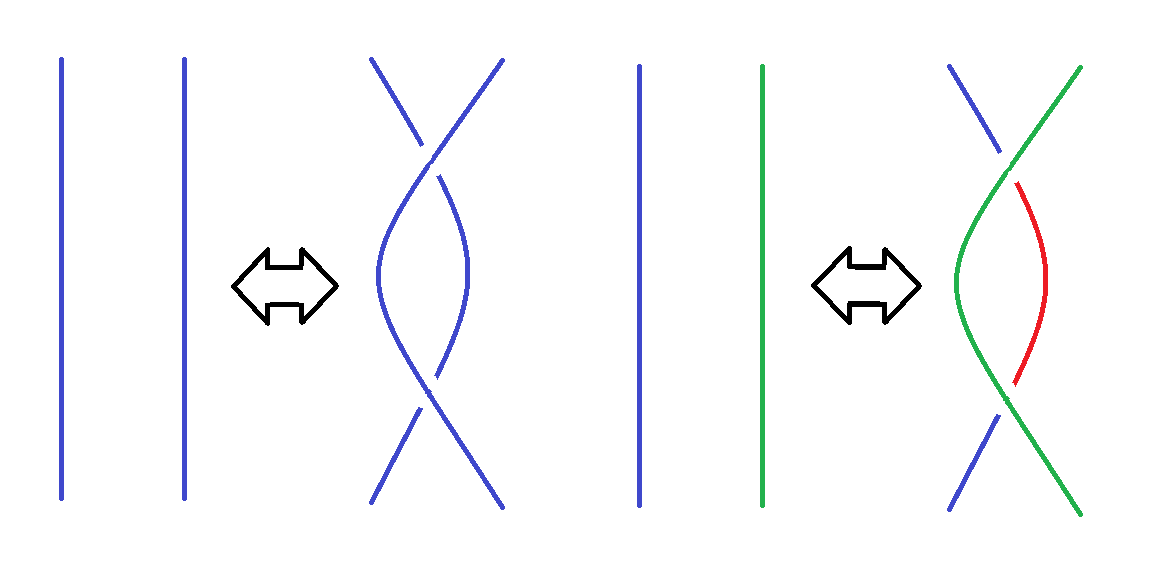
\includegraphics[scale=\ds]{t2-c}
    \caption{type-II}
    \label{fig:t2-c}
  \end{figure}

  Finally, for type-III moves there are several cases based on
  the colors of the strands entering. We will demonstrate
  three such cases, given in Figure~\ref{fig:t3-c}, and the rest are similar.
  \begin{figure}
    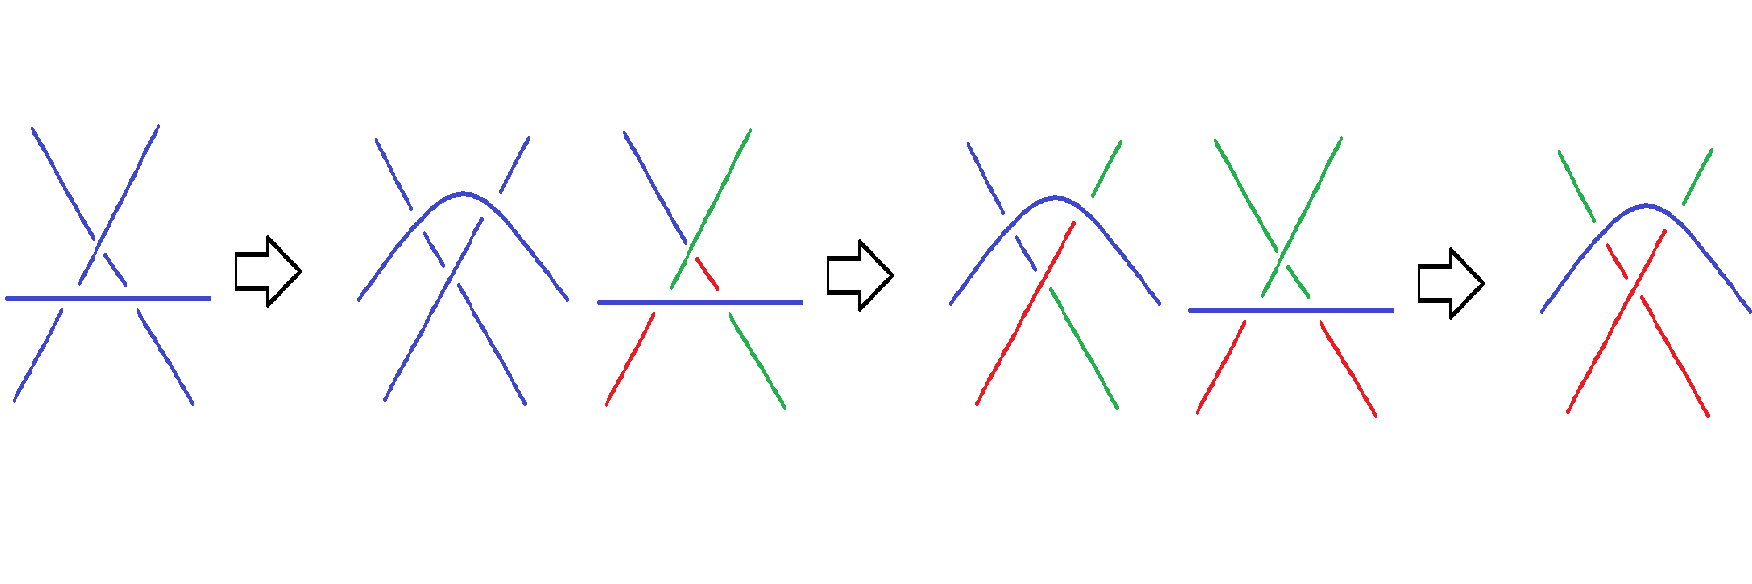
\includegraphics[scale=\ds]{t3-c}
    \caption{type-III}
    \label{fig:t3-c}
  \end{figure}

  Thus if a diagram $D$ for a knot $K$ has a $3$-coloring, then
  any diagram for $K$ has a $3$-coloring. Therefore $3$-colorability
  is a knot invariant.
\end{proof}

An immediate consequence of this is that the unknot and the trefoil
knot are in fact not identical. We can see this because the unknot
is not tricolorable as it only has a single arc. However, the
trefoil can be colored as in Figure~\ref{fig:trefoil-c}.

\begin{figure}
  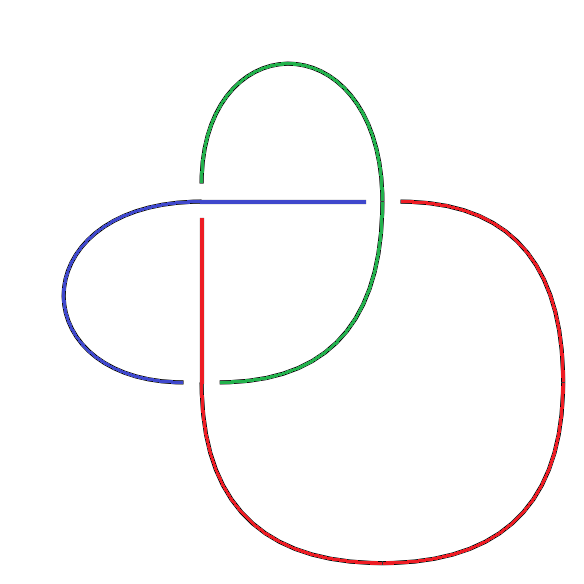
\includegraphics[scale=\ds]{trefoil-c}
  \caption{Colored trefoil}
  \label{fig:trefoil-c}
\end{figure}

\section{The Knot Group}
\label{sec:knot-group-d_6}

The definition of $3$-coloring is a perfectly valid definition for a knot
invariant. However, it is defined in terms of diagrams and, as such,
we had to do some extra work with the Reidmeister moves to show that it
was indeed an invariant. Ideally, there would be an equivalent definition
of coloring that does not involve diagram, but rather, only involves
the knot and its embedding into $S^3$. Then it may be easier to tease
out what topological properties are being captured by $3$-coloring.

It turns out that there is a way to define $3$-coloring in this manner
and it has to do with a construction called the knot group. Ones first
instinct to get a group out of a knot might be to take the fundamental
group. However, since all knots are copies of $S^1$, the fundamental group
for any knot is $\bb{Z}$. As such, we have to take advantage of its
ambient space.

\begin{definition}
  Let $K$ be a knot. Then the \textit{knot group} of $K$ is the fundamental
  group $\pi_1(S^3\setminus K,*)$.
\end{definition}

This definition makes use of the embedding of the knot into $S^3$ and
so will not be identical for all knots. Naturally, we need a way
to calculate the knot group. We can do this using what is called
the \textit{Wirtinger presentation}~\cite{hatcher}.

\begin{theorem}[Wirtinger]
  Let $K$ be a knot and $D$ a diagram for $K$. Choose an
  orientation for $D$. Let $x_1,\ldots,x_n$
  denote the arcs of $D$ and, for each crossing, give a relation
  $r_1\ldots, r_m$ such that $r_i \equiv (x_ix_jx_i^{-1}=x_k)$ where, when approaching
  $x_k$ is the arc leaving the crossing, the top arc is $x_i$ and the bottom
  arc entering is $x_j$. Then the knot group of $K$ has the presentation
  \[
    \pi_1(S^3\setminus K,*)\cong \langle x_1,\ldots, x_n| r_1,\ldots,r_m\rangle
  \]
\end{theorem}

Now we give a couple of examples.

\begin{example}
  The knot group of the unknot is
  \[
    \langle x_1 |\rangle \cong \bb{Z}
  \]
  as there are no crossings and only a single arc.
\end{example}

\begin{example}
  The trefoil knot has three crossings and three arcs. Label it as
  shown in Figure~\ref{fig:annotated-trefoil}. Then the Wirtinger presentation
  of the knot group of the trefoil is
  \[
    \langle x_1,x_2,x_3|x_1x_2x_1^{-1}=x_3,x_3x_1x_3^{-1}=x_2,x_2x_3x_2^{-1}=x_1\rangle
  \]
  However, the presentation of this group can be simplified to the
  form
  \[
    \langle x_1,x_2| x_1x_2x_1=x_2x_1x_2\rangle
  \]
\end{example}

\begin{figure}
  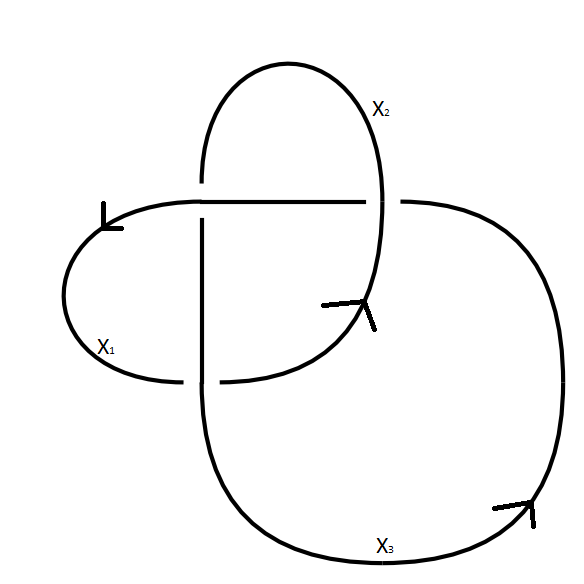
\includegraphics[scale=\ds]{annotated-trefoil}
  \caption{Annotated Trefoil}
  \label{fig:annotated-trefoil}
\end{figure}

The knot group gives us another invariant of knots. Unfortunately,
presentations of groups can be rather difficult to work with.
Thus, to make the problem more tractable, we instead look
at homomorphisms from the knot group to finite groups as these
will be determined by where we send generators. This is
how we will redefine coloring in terms of the knot group~\cite{quickfox}.

\begin{definition}
  Let $K$ be a knot and $G$ the corresponding knot group. Then a
  \textit{Fox $3$-coloring} of $K$ is a homomorphism $\rho$ from
  $G$ to the symmetry group $D_6$ of an equilateral triangle. We say that
  $\rho$ is a \textit{non-trivial coloring} if $\rho$ is surjective.

  Thus a knot $K$ is \textit{Fox $3$-colorable} if there exists a nontrivial
  Fox $3$-coloring.
\end{definition}

Now a couple of examples using our prior work.

\begin{example}
  Recall that the knot group of the unknot is $\bb{Z}$. Since
  $\bb{Z}$ has only a single generator, it is not possible to
  create a surjective homomorphism onto $D_6$ as $D_6$ has
  two generators.
\end{example}

\begin{example}
  As we calculated above, the knot group for the trefoil is
  \[
    \langle x_1,x_2| x_1x_2x_1=x_2x_1x_2\rangle.
  \]
  Similarly, we can write a presentation of $D_6$ as
  \[
    \langle r,s| r^3=1, s^2=1,srsr=1\rangle.
  \]
  This gives us two non-trivial Fox $3$-colorings of the trefoil.
  The first sends $x_1$ to $r$ and $x_2$ to $s$ and the
  other swaps which generator is sent to which generator.
\end{example}

As was implied by the prior examples, there is a relation between
Fox $3$-coloring and the $3$-colorability of knots. In fact, it turns
out that they are the same.

\begin{theorem}
  A knot $K$ has a $3$-coloring if and only if there is a
  Fox $3$-coloring of $K$.
\end{theorem}

A proof of this theorem can be found in~\cite{medwid}. 
The proof there relates two notions of coloring using
the Wirtinger presentation to marry the conditions necessary
for the existence of a $3$-coloring and the existence of a Fox
$3$-coloring.

\section{$n$-coloring}
\label{sec:n-coloring}

What are the benefits of looking at $3$-coloring through
the lens of Fox $3$-coloring? Unlike with coloring diagrams,
it is immediate that Fox $3$-coloring is a knot invariant
as the fundamental group is invariant under homotopy equivalence.
So Fox $3$-coloring must be invariant under ambient isotopy as well. Another benefit
is that it is more readily apparent how we can further
extend Fox $3$-coloring than extending $3$-coloring. From
the definition of $3$-coloring, there is some ambiguity that
would need to be sorted out about precisely what rules need
to change. For example, one of our conditions was that either
all colors appear at a crossing or none. Since a crossing has
at most three arcs entering it would not be possible to have
all colors meet if we were attempting to color with more than three.

This is avoided with Fox $3$-coloring. The only choice we made
was that we are looking at homomorphisms to $D_6$. We could
very easily have chosen any finite group and gotten the
same nice structure that we had above. The reason that
$D_6$ is the group used for Fox $3$-coloring is that it is
the group of symmetries of the triangle. We can
define the Fox $n$-coloring similarly. Let $D_{2n}$ be
the symmetry group of a regular $n$-gon.

\begin{definition}
  Let $G$ be the knot group of a knot $K$. Then
  a \textit{Fox $n$-coloring} of $K$ is a homomorphism $\rho: G\rightarrow D_{2n}$
  where $\rho$ is called a \textit{non-trivial $n$-coloring} if $\rho$ is
  surjective.
\end{definition}

We can also extend the notion of coloring that we started
with. However, it does take more effort. Instead of choosing
the colors that we did when originally defining $3$-coloring,
we could just as easily have used numbers instead. Then,
instead of requiring that each crossing either have all three
colors appear or only a single color appear, would be equivalent to each
crossing satisfying the equation
\[
  2x-y-z\equiv 0 \mod 3
\]
where the arcs of the crossing are labeled as in Figure~\ref{fig:numcolor}.

\begin{figure}
  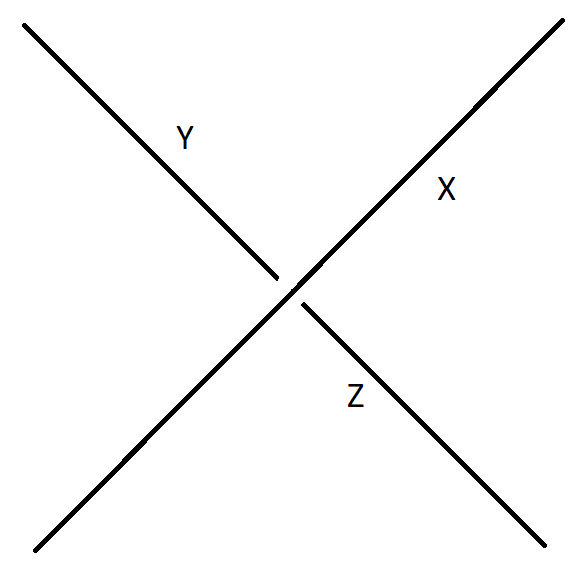
\includegraphics[scale=\ds]{numcolor}
  \caption{Colored Crossing}
  \label{fig:numcolor}
\end{figure}

In this form, it is more apparent how we could extend $3$-coloring
to arbitrary $n$ by simply replacing the modulus. Going back
to our initial example of a knot, the figure-eight knot, we have
an example of a knot that is not $3$-colorable but is 5-colorable
as shown in Figure~\ref{fig:figure-eight-c}.

\begin{figure}
  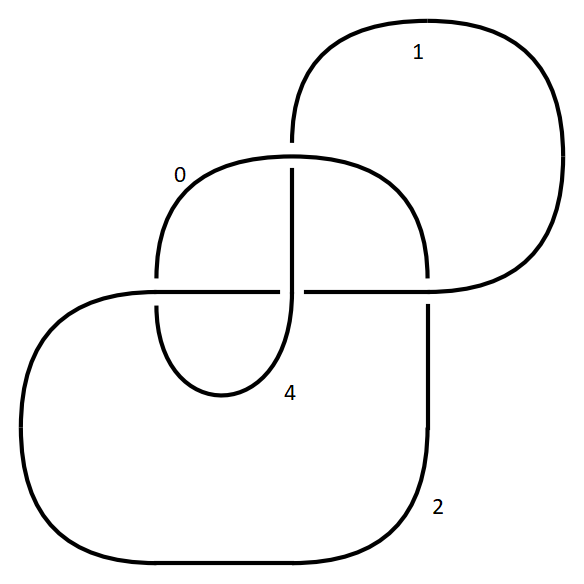
\includegraphics[scale=\ds]{figure-eight-c}
  \caption{Figure-eight 5-coloring}
  \label{fig:figure-eight-c}
\end{figure}

\pagebreak

\begin{thebibliography}{99}

\bibitem{hatcher}  Hatcher, A., \textit{Algebraic Topology,}
  Cambridge University Press, Cambridge, 2001. 
  
\bibitem{Livingston}  Livingston, C., \textit{Knot Theory,}
  Mathematical Association of America, Washington DC, 1996. 
  
\bibitem{medwid}  Medwid, M., \textit{Generalized $P$-Colorings of Knots,}
  Bowling Green University, 2014.
  
\bibitem{Poonen}  Poonen, Bjorn. Undecidable Problems: a Sampler, in
  \textit{Interpreting GöDel}, pp. 211241., doi:10.1017/cbo9780511756306.015.
  
\bibitem{quickfox}  Fort, M. K., and Fox R.H.,
  \textit{A Quick Trip Through Knot Theory}, in Topology of 3-Manifolds and
  Related Topics, Dover Publications, Mineola, 2010.
\end{thebibliography}

\end{document}
